\documentclass[aspectratio=1610]{beamer}
\usetheme{boxes}
\usecolortheme{crane}
\usepackage{amsmath,amsfonts}
\usepackage{algpseudocode}
\usepackage{multicol}
\usepackage{pgfplots}
\pgfplotsset{compat=1.15}
\usepackage{mathrsfs}
\usetikzlibrary{arrows}
\usepackage{listings}


%-------------------------------------------------------------------
%	 TITLE SLIDE
%-------------------------------------------------------------------


\begin{document}

% -------------------------------------------------------------------
% Lesson 3
% -------------------------------------------------------------------
\section{Data Structures and Algorithms}

\begin{frame}
\begin{center}
\Huge Lesson 3\\~\\
\textbf{Data Structures and Algorithms DSA}
\end{center}
\end{frame}


\begin{frame}
\frametitle{Lesson 3}

\huge In this lesson we will talk about:
\begin{itemize}
	\item \alert{data structures}
	\item \alert{algorithm design}
	\item \alert{algorithm efficiency}
	\item \alert{searching and sorting algorithms}
\end{itemize}
\end{frame}


\begin{frame}{Lesson 3}{}
\begin{center}
\Huge \textbf{Data Structures}
\end{center}
\end{frame}


\begin{frame}{Lesson 3}{}
\Huge{What is a data structure?}\\~\\
\includegraphics[scale=0.80]{Images/ds}
\end{frame}


\begin{frame}{Lesson 3}{}
\LARGE
\textbf{Data Structures}\\~\\
\begin{itemize}
    \item How do we \textbf{organize} data
    \item For a very \textbf{efficient} access
\end{itemize}

It's a collection of data values, and the relationships among these values
\end{frame}


\begin{frame}{Lesson 3}{}
\LARGE
\textbf{Data Structures}
\begin{center}
\includegraphics[scale=0.80]{Images/data_structures}
\end{center}
\end{frame}



\begin{frame}
\frametitle{Lesson 3}
\LARGE 
\textbf{Linear Data Structures: Arrays, Queues, Stacks}\\~\\
\begin{itemize}
	\item Elements are arranged sequentially, one after the other
	\item The first element added will be the first one to be accessed or removed, and the last element added will be the last one to be accessed or removed
	\item Can have either fixed or dynamic sizes
	\item Offer very efficient data access
\end{itemize}
\end{frame}


\begin{frame}
\frametitle{Lesson 3}
\LARGE 
\textbf{Non-linear Data Structures: Trees, Graphs}\\~\\
\begin{itemize}
	\item Elements are arranged hierarchical
	\item We can’t traverse all the elements in a single run only
	\item There are multiple levels which we must traverse
	\item It is more difficult to implement
\end{itemize}
\end{frame}


\begin{frame}{Lesson 3}{}
\LARGE
\textbf{Data structures}
\begin{itemize}
    \item Sets
    \item Arrays and Matrices
    \item Stacks
    \item Queues
    \item Linked lists
    \item Trees
    \item Graphs
\end{itemize}
\end{frame}


\begin{frame}{Lesson 3}{}
\begin{center}
\Huge Sets
\end{center}
\end{frame}


\begin{frame}{Lesson 3}{Sets}
\LARGE
\textbf{Sets}\\~\\
A set is usually a \textbf{collection} of different things, fixed in size. Sets can also change size, usually when an algorithm will perform modifications against the set. We call these dynamic sets. These sets can change in size, grow or shrink, basically change over the time.
\end{frame}


\begin{frame}{Lesson 3}{Sets}
\Huge{But what is a set?}\\~\\
\end{frame}


\begin{frame}{Lesson 3}{Sets}
\LARGE
\textbf{Sets}\\~\\
The basic, fundamental data structure: \{1,2,4,51,9\}
\begin{itemize}
    \item mathematical set
    \item unchanging, unique elements, no duplicates
    \item contains a fixed number of elements: finite set
    \item or it can contain an infinite number of elements
\end{itemize}

\end{frame}


\begin{frame}{Lesson 3}{Sets}
\LARGE
\textbf{For example a set of polygons}
\begin{center}
\includegraphics[scale=0.10]{Images/set}
\end{center}
\end{frame}


\begin{frame}{Lesson 3}{Sets}
\LARGE
\textbf{Sets}\\~\\
A set is a \textbf{mathematical model} of a collection of different things. A set contains elements or members, which can be mathematical objects of any kind numbers, symbols, points in space, lines, other geometrical shapes, variables, or even other sets.

\end{frame}


\begin{frame}{Lesson 3}{Sets}
\LARGE
\textbf{Sets, examples}\\~\\
\begin{itemize}
    \item \{white, blue, red, yellow\}
    \item The empty set \{\}
    \item Natural numbers: $\mathbb{N} = \{0, 1, 2, 3, \ldots\}$
    \item Natural numbers except 0: $\mathbb{N^*} = \{1, 2, 3, \ldots\}$
    \item Integers: $\mathbb{Z} = \{\ldots, -3, -2, -1, 0, 1, 2, 3, \ldots\}$
    \item Positive integers: $\mathbb{Z_+} = \{0, 1, 2, 3, \ldots\}$
\end{itemize}
\end{frame}



\begin{frame}{Lesson 3}{Sets}
\LARGE{\textbf{\{1,2,3,4\}}}\\~\\
\LARGE
Defines a list of elements, using a simple enumeration notation (Roster notation) between curly brackets, separated by commas.
\end{frame}


\begin{frame}{Lesson 3}{Sets}
\LARGE
\textbf{Basic Operations on Sets}\\~\\
\begin{itemize}
    \item Insert - add a new element to a set
    \item Delete - remove an element from a set
    \item Test - if element X belongs to a set or not 
\end{itemize}

A dynamic set which supports all these basic operations: \textbf{a dictionary} 
\end{frame}


\begin{frame}{Lesson 3}{Sets}
\begin{center}
\includegraphics[scale=0.45]{Images/numbers3}
\end{center}
\end{frame}


\begin{frame}{Lesson 3}{Sets}
\begin{center}
\includegraphics[scale=0.14]{Images/NZQRC}
\end{center}
\end{frame}


\begin{frame}{Lesson 3}{Sets}
\LARGE
\textbf{Advantages}\\~\\
Perform operations on a collection of elements in a very \textbf{efficient} and \textbf{organized} manner
\end{frame}


\begin{frame}{Lesson 3}{Sets}
\LARGE
\textbf{Conclusions}\\~\\
Sets are basic, fundamental data structures, with:
\begin{itemize}
    \item unique elements
    \item no duplicates
    \item unchanging 
    \item fixed or infinite number of elements
\end{itemize}

\end{frame}


\begin{frame}{Lesson 3}{Sets}
\LARGE
\textbf{Im confused. Does it mean a set is similar to a Python set? Or what is the difference?}
\end{frame}


\begin{frame}{Lesson 3}{Sets}
\LARGE
\textbf{Sets vs. Python Set}\\~\\
In computer science (CS), a set is an abstract data type that can store unique values, without any particular order. It is a computer implementation of the mathematical concept of a finite set.
\end{frame}



\begin{frame}{Lesson 3}{Sets}
\LARGE
\textbf{Mathematical vs. Python Sets}\\~\\
\begin{itemize}
    \item Mathematical finite set: \{1,2,3,4\}
    \item Python set: S = \{1,2,3,4\}
\end{itemize}
\end{frame}



% %%%%%%%%%%%%%%%%%%%%%%%%%%%%%%%%%%%%%%%%%%%%%%%%%%%%
% Arrays
% %%%%%%%%%%%%%%%%%%%%%%%%%%%%%%%%%%%%%%%%%%%%%%%%%%%%
\begin{frame}{Lesson 3}{}
\begin{center}
\Huge Arrays
\end{center}
\end{frame}

\begin{frame}{Lesson 3}{Arrays}
\LARGE
\textbf{Arrays}\\~\\
In computer science, an \textbf{array} is a data structure consisting of a collection of elements, each identified by an \textbf{index} or a \textbf{key}. The simplest type of such data structure is a linear array, the one-dimensional array.
\end{frame}


\begin{frame}{Lesson 3}{Arrays}
\begin{center}
\includegraphics[scale=0.17]{Images/array2.png}
\end{center}
\end{frame}



\begin{frame}{Lesson 3}{Arrays}
\LARGE
\textbf{Arrays}\\~\\
Arrays are among the oldest and most important data structures, and are used by almost every program and programming language. They are also used to implement many other data structures, such as lists.
\end{frame}


\begin{frame}{Lesson 3}{Arrays}
\LARGE
\textbf{Arrays}\\~\\
Arrays are useful because the element indices can be computed at \alert{run time}. Among
other things, this feature allows a single iterative statement to process arbitrarily many
elements of an array. For that reason, the elements of an array data structure are required
to have the same size and should use the same data representation. 
\end{frame}



\begin{frame}{Lesson 3}{Arrays}
\LARGE
\textbf{Run-time?}\\~\\
Runtime, run time, or execution time is the final phase of a computer program's life cycle,
in which the code is being executed on the computer's central processing unit (CPU) as
machine code. In other words, "runtime" is the running phase of a program.
\end{frame}



\begin{frame}{Lesson 3}{Arrays}
\Large
\textbf{Remember this? From source code to executable}\\~\\ 
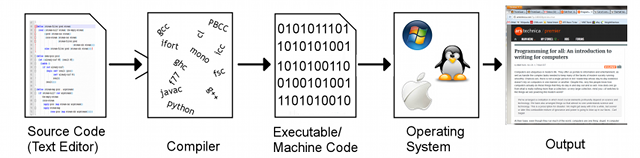
\includegraphics[scale=0.65]{Images/CompilationChain}
\end{frame}



\begin{frame}{Lesson 3}{}
\LARGE
\textbf{Basic Array Operations}\\~\\
\begin{itemize}
	\item traversal of an array
	\item access element X in an array
	\item searching element X in an array
	\item sorting an array
\end{itemize}
\end{frame}



\begin{frame}{Lesson 3}{Arrays}
\Large
\textbf{Example 1: Traversing the array A}\\~\\

\label{getArray}
\begin{algorithmic}[1]
\Procedure{getArray}{$A$} \Comment{Returns the max value in A}
\State $L\gets length(A)$
\For{\texttt{i=0 to L-1}}
    \State print $A[i]$
\EndFor
\EndProcedure
\end{algorithmic}
\end{frame}


\begin{frame}[fragile]
\LARGE
\textbf{Traversing the array}\\~\\
\Large
\begin{lstlisting}[language=Python]
A = [1, 2, 3, 4, 5, 6, 7,8,9]

# Traversing the array
for element in A:
    print(element, end=" ")
    
\end{lstlisting}
\end{frame}



\begin{frame}[fragile]
\LARGE
\textbf{Traversing the array}\\~\\
\Large
\begin{lstlisting}[language=Python]
A = [1, 2, 3, 4, 5, 6, 7,8,9]

# Traversing the array
for i in range(len(A)):
    print(A[i], end=" ")
    
\end{lstlisting}
\end{frame}


\begin{frame}{Lesson 3}{Arrays}
\Large
\textbf{Example 2: Find the max value in the array A}\\~\\

\label{MaxArray}
\begin{algorithmic}[1]
\Procedure{MaxArray}{$A$} \Comment{Returns the max value in A}
\State $N\gets length(A)$
\State $MAX\gets A[0]$
\For{\texttt{from i=1 to N-1}}
\If {$A[i] > MAX$}
    \State \textbf{$MAX = A[i]$} \Comment{The MAX is A[i]}
\EndIf
\EndFor
\State \Return $MAX$
\EndProcedure
\end{algorithmic}
\end{frame}



\begin{frame}{Lesson 3}{Arrays}
\Large
\textbf{Example 3: Search element X in array A}\\~\\
\label{SearchArray}
\begin{algorithmic}[1]
\Procedure{SearchArray}{$A$} \Comment{Returns the max value in A}
\State $X\gets MyElement$
\State $N\gets length(A)$
\For{\texttt{from i=0 to N-1}}
\If {$X = A[i]$}
    \State \Return {$i$}  \Comment{The index for my match}
\EndIf
\EndFor
\State \Return -1 \Comment{otherwise return -1}
\EndProcedure
\end{algorithmic}
\end{frame}



\begin{frame}{Lesson 3}{}
\LARGE
\textbf{There are numerous applications of arrays}\\
\begin{itemize}
    \item Storing data in databases. Storing a list of customer names.  
    \item Traffic Management.Traffic management systems use arrays to track vehicles and
    their flow. By analyzing data stored in arrays, traffic control centers can implement
    efficient signal timings and manage congestion effectively.
\end{itemize}
\end{frame}



\begin{frame}{Lesson 3}{Arrays}
\LARGE
\begin{itemize}
    \item Financial Analysis. It keeps track of various financial instruments, including stocks, bonds, and mutual funds. By organizing data in arrays, companies can perform analyses and make predictions easier 
    \item Machine Learning. Machine learning algorithms often accept arrays as input, helping to train models and make predictions.
\end{itemize}
\end{frame}



% %%%%%%%%%%%%%%%%%%%%%%%%%%%%%%%%%%%%%%%%%%%%%%%%%%%%
% Matrices
% %%%%%%%%%%%%%%%%%%%%%%%%%%%%%%%%%%%%%%%%%%%%%%%%%%%%
\begin{frame}{Lesson 3}{Matrices}
\begin{center}
\Huge Matrices
\end{center}
\end{frame}


\begin{frame}{Lesson 3}{Matrices}
\LARGE
\textbf{What is a matrix?}\\~\\
In mathematics, a matrix (pl.: matrices) is a rectangular array or table of numbers,
symbols, or expressions, with elements or entries arranged in rows and columns, which is
used to represent a mathematical object or property of such an object.
\end{frame}


\begin{frame}{Lesson 3}{Matrices}
\LARGE
\textbf{Matrices}
\begin{center}
\includegraphics[scale=0.14]{Images/matrices2}
\end{center}
\end{frame}


\begin{frame}{Lesson 3}{Matrices}
\LARGE
\textbf{Matrices}
\begin{center}
\includegraphics[scale=0.10]{Images/Matrix}
\end{center}
\end{frame}


\begin{frame}{Lesson 3}{Matrices}
\LARGE
\textbf{Basic Matrix Operations}\\~\\
\begin{itemize}
	\item access X element in a matrix
	\item traversal of a matrix
	\item searching a matrix
	\item sorting a matrix
\end{itemize}
\end{frame}




\begin{frame}[fragile]
\LARGE
\textbf{Accessing the elements of a matrix}\\~\\
\Large
\begin{lstlisting}[language=Python]
A = [[1, 2, 3], [4, 5, 6], [7,8,9]]

# Accessing certain elements in a matrix
print("1st element of 1st row:", A[0][0])
print("2nd element of the 2nd row:", A[1][2])
print("2nd element of 3rd row:", A[2][1])
\end{lstlisting}
\end{frame}



\begin{frame}[fragile]
\LARGE
\textbf{Traversing the matrix}\\~\\
\Large
\begin{lstlisting}[language=Python]
A = [[1, 2, 3], [4, 5, 6], [7,8,9]]

# Traversing the matrix
for row in A:
    # Traversing the matrix
    for x in row:
        print(x, end=" ")
    print()
\end{lstlisting}
\end{frame}


\begin{frame}{Lesson 3}{Matrices}
\LARGE
\textbf{There are numerous applications of matrices}\\
\begin{itemize}
    \item Encryption: Matrices encrypt data into unreadable formats and decode it for secure communication. 
    \item Computer Graphics: transformations like scaling, rotation, and translation of objects in 2D and 3D graphics
    \item Machine Learning: fundamental data structures for neural networks  
\end{itemize}
\end{frame}


\begin{frame}{Lesson 3}{Matrices}
\LARGE
\begin{itemize}
	\item Economics and Business: optimize business operations like supply chains and financial forecasting
	\item Navigation Systems: GPS systems use matrices to calculate positions, distances, and directions in 2D and 3D space.
	\item Weather Prediction: Matrices solve systems of differential equations to model and predict climate and weather patterns
\end{itemize}
\end{frame}


\end{document}
